Dans cette partie du rapport, nous ne suivrons pas l'ordre des
questions par faute de temps. Nous r\'esumerons plut\^ot les
différentes \'etapes de nos deux impl\'ementation \verb'i-java'
(\emph{i.e} impl\'ementation en \verb'JAVA(JDK8)') et \verb'i-c'
(\emph{i.e} impl\'ementation en \verb'C') et analyserons bri\`evement
quelques r\'esultats.\\

Nous avons chacun impl\'ement\'e une version diff\'ente de
\verb'COUT1' et \verb'SOL1'. Nous nous int\'eresserons \`a
l'impl\'ementation des autres algorithmes et \`a une analyse plus
pouss\'ee des r\'esultats dans le temps imparti jusqu'\`a la
soutenance le 28 novembre 2016.\\\\

\subsection{(VALETTE) \texttt{i-c}}
Les deux fonctions \texttt{COUT1} et \texttt{SOL1} sont programm\'ees
en C et contenues dans le fichier \texttt{cout\_sol\_1.c} (en-t\^ete :
\texttt{cout\_sol\_1.h}). Le jeu d'essai est fourni dans le fichier
\texttt{prod.c}. Le \texttt{Makefile} fourni permet de compiler tous
les fichiers du projet avec l'utilitaire \texttt{make}, sur toute
version de \texttt{gcc} supportant le standard C11.\\\\

\begin{figure*}[h]
\centering
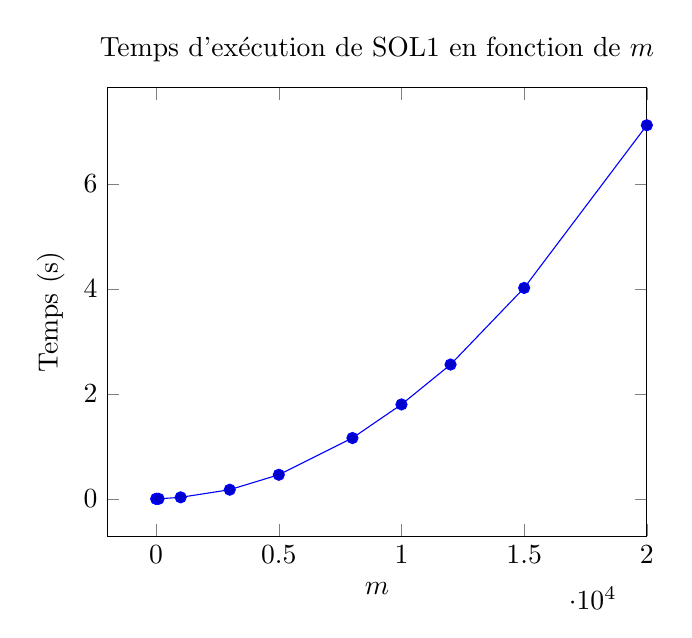
\begin{tikzpicture}
\begin{axis}[xmax=20000, xlabel={$m$}, ylabel={Temps (s)}, title={Temps d'exécution de SOL1 en fonction de $m$}]
\addplot coordinates {
(4,0.001) (10,0.001) (100,0.0015) (1000,0.03) (3000,0.175) (5000,0.46) (8000,1.16) (10000,1.8) (12000,2.56) (15000,4.02) (20000,7.12)};
\end{axis}
\end{tikzpicture}
\end{figure*}

Pour la fonction \texttt{COUT1}, la plus grande valeur de $m$
traitable en un temps raisonnable (environ $7$ secondes) est $20\ 000$
(\texttt{Inst\_20000\_64.adn}). Il en est de m\^eme pour la fonction
\texttt{sol1}. (Caract\'eristiques m\'emoire : $8$Go)

\subsection{(BEN KIRANE) \texttt{i-java}}
Avec une volont\'e de faciliter la lecture du code et sa
r\'eutilisation, le langage choisi dans cette partie est
\texttt{JAVA}. On peut dans un premier temps \^etre perplexe
vis-\`a-vis de la complexit\'e en m\'emoire et en temps d'un programme
orient\'e objet (OO) mais les premiers essais -- je n'ai pas encore
test\'e les instances dont les cha\^ines font plus de $10\ 000$
nucl\'eotides -- sont plut\^ot satisfaisants et ne s'\'ecartent pas trop
de la version \verb'i-c'. 

Cependant, il me reste bien entendu \`a am\'eliorer le code, \`a le
tester sur de plus grandes instances et impl\'ementer les autres
algorithmes de la partie th\'eorique (3).  \newpage Dans cette
premi\`ere phase d'impl\'ementation, une importance particuli\`ere \`a
\'et\'e donn\'ee \`a la modularit\'e et \`a l'articulation des objets
manipul\'es :
\begin{description}
\item[instances] La classe \verb'PaireDeSequence' permet de manipuler
  les instances.
\item[p\'enalit\'es] La classe abstraite \verb'AbstractPenalites' et
  sa premi\`ere \'extension \verb'PenalitesInteger' permettent de
  manipuler les p\'enalit\'es de correspondances attribu\'ees \`a des
  couples de nucl\'eotides donn\'es, avec notamment un format de
  fichier facilitant les tests.
\item[optimisation] La classe abstraite \verb'AbstractCompare' et sa
  premi\`ere \`extension \verb'CompareInteger1' permettent de
  r\'esoudre le probl\`eme pos\'e \`a la premi\`ere sous-partie de la
  partie th\'eorique.
\item[tests] Les classes \verb'Afficher', \verb'AfficherPenalites' et
  \verb'TestCompare1' illustrent les trois points d\'ecrits ci-dessus.
\end{description}
Enfin on pourra se r\'ef\'erer \`a la documentation
(\verb'i-java/doc') et aux sources (\verb'i-java/src') pour mieux
comprendre l'impl\'emenation de ce qui \`a \'et\'e trait\'e.
%%% Local Variables:
%%% mode: latex
%%% TeX-master: "rapport"
%%% End: